\clearpage
\chapter{\textbf{Vorwissen}}\label{chap:Vorwissen}
\addtocontents{toc}{\vspace{0.8cm}}
Im Folgenden werden ein paar Grundlagen und Definitionen erläutert. Sie sollen das Verständnis der Algorithmen in Kapitel \ref{chap:Lokalisierung - Lösungsansätze} ermöglichen und fördern. 


\section{bestimmbare Positionen}\label{sec:bestimmbare Positionen}
\addtocontents{toc}{\vspace{0.8cm}}
Die Position eines sich auf dem Boden bewegenden mobilen Roboters, in Bild \ref{fig:1a_dd}  eines sog. Differential Drive Roboters, kann angegeben werden durch 
$P=\mathbf{\begin{psmallmatrix}
x & y & \psi
\end{psmallmatrix}}^\intercal$.
Hierbei bezieht sich $x$ auf die Position gepeilt auf die x-Achse, $y$ die Position gepeilt auf die y-Achse und $\psi$  den Winkel zwischen der Ausrichtung des Roboters und der x-Achse. Die Literatur bezeichnet die erhaltene Position im Fall eines bodengebundenen Roboters als eine 2D Position.\\
Zur Positionsbestimmung eines UAVs kommt im Falle einer 3D Positionsbestimmung eine weitere Achse hinzu, sodass die 3D Position angegeben werde kann durch
$P=\mathbf{\begin{psmallmatrix}
x & y & z & \psi
\end{psmallmatrix}}^\intercal$.
Die zusätzliche Variable $z$ bezeichnet hierbei die Position des Roboters gepeilt auf die z-Achse. (siehe Bild \ref{fig:1b_uav})\\
Eine weitere Darstellung der Position eines UAVs ist die 6D Position. Hierbei kommen zu der eben besprochenen 3D Position zwei Winkel hinzu, wodurch die 6D Position angegeben werden kann durch
$P=\mathbf{\begin{psmallmatrix}
x & y & z & \psi & \theta & \varphi
\end{psmallmatrix}}^\intercal$.
Dies folgt einer Konvention der Luft-und Raumfahrt, dem Schiffbau und dem Automobilbau \cite{website:cosmos-indirekt}, wonach die Reihenfolge der Eulerschen Winkel in Gier-, Nick-, und Rollwinkel (engl. \textit{yaw, pitch, roll}) festgelegt ist. (siehe Bild \ref{fig:1c_euwinkel}) Der Winkel $\psi$ beschreibt folglich den Gierwinkel, $\theta$ den Nickwinkel und $\varphi$ den Rollwinkel. % Koordinatensystemsbilder für Positionen
\mbox{}
\begin{figure}
  \begin{subfigure}[t]{.3\textwidth}
    \centering
    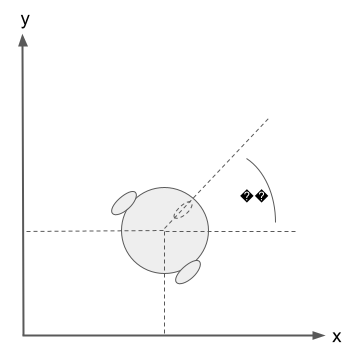
\includegraphics[width=.9\linewidth]{pic/vorwissen/1a_diffdrive.png}
    \caption{Position eines \textit{Differential Drive} Roboters}
    \label{fig:1a_dd}
  \end{subfigure}\hfill
  \begin{subfigure}[t]{.3\textwidth}
    \centering
    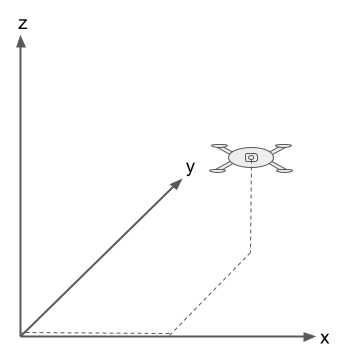
\includegraphics[width=.9\linewidth]{pic/vorwissen/1b_uav.png}
    \caption{Position eines UAV im dreidimensionalen Raum}
    \label{fig:1b_uav}
  \end{subfigure}\hfill
  \begin{subfigure}[t]{.3\textwidth}
    \centering
    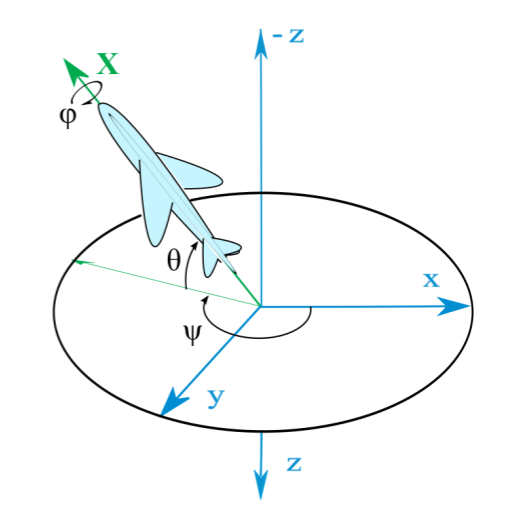
\includegraphics[width=.9\linewidth]{pic/vorwissen/1c_eulerwinkel.png}
    \caption{Konvention für Eulersche Winkel \cite{website:cosmos-indirekt-grafik}}
    \label{fig:1c_euwinkel}
  \end{subfigure}
  \label{fig:positionen}
\end{figure}
\mbox{}


\section{Kartenrepräsentation}\label{sec:Kartenrepräsentation}
\addtocontents{toc}{\vspace{0.8cm}}
Zur Positionsbestimmung in einer Karte ist die Auswahl der Kartenrepräsentation maßgebend. In der Kartendarstellung wird unterschieden zwischen einem topologischen- und einem metrischen Gerüst für eine Karte.\\
Bei einem topologischen Rahmen werden nur die Orte und dessen Beziehungen berücksichtigt, sodass die Karte ein Graph ist, bestehend aus Knoten, die die Orte repräsentieren und Bögen, die die Verbindungen der Orte darstellen. In einem metrischen Gerüst für eine Karte wird die räumlich-, Koordinatensystem-basierte Darstellung der Karte verwendet. Die Objekte innerhalb der Karte haben hierbei genaue Koordinaten.\\
Die in dieser Arbeit zumeist verwendeten Karten nutzen sogenannte \textit{Occupancy Grid Maps}. Hierbei wird ein Gitter mit definierter Masche auf die Karte gelegt. Befindet sich ein Objekt in der Karte, so wird jedes Gitterkästchen in dem sich das Objekt befindet als besetzt (engl. \textit{occupied}) gewertet und schwarz eingefärbt, wie in der Bilderreihe \ref{fig:occupanygridmap} dargestellt. So können die für eine Karte benötigten Datenmengen kontrolliert und eingegrenzt werden.\\
Im dreidimensionalen Raum können Occupancy Grid Maps ebenfalls eingesetzt werden. Der Raum kann dann nicht mehr nur mithilfe von zweidimensionalen Kästchen diskretisiert werden, sondern muss durch Würfel, sogenannte \textit{Voxel} eingeteilt und dargestellt werden.
\mbox{} % Biler Occupancy Grid Map 
\begin{figure}
  \begin{subfigure}[t]{.3\textwidth}
    \centering
    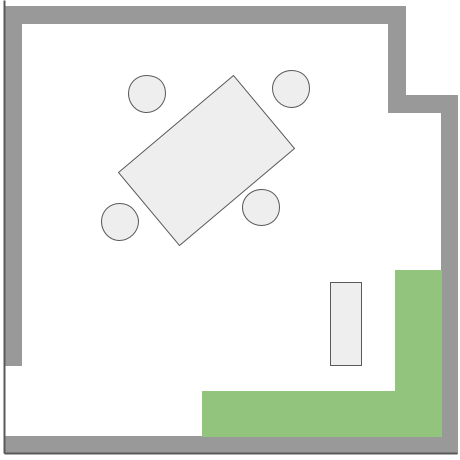
\includegraphics[width=.9\linewidth]{pic/vorwissen/2a_karte.png}
    \caption{Draufsicht eines Raumes}
  \end{subfigure}\hfill
  \begin{subfigure}[t]{.3\textwidth}
    \centering
    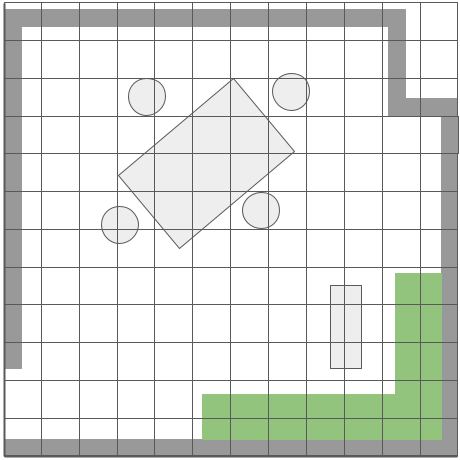
\includegraphics[width=.9\linewidth]{pic/vorwissen/2b_kartengitter.png}
    \caption{Einteilen des Raumes in gleichmäßig große Kästchen}
  \end{subfigure}\hfill
  \begin{subfigure}[t]{.3\textwidth}
    \centering
    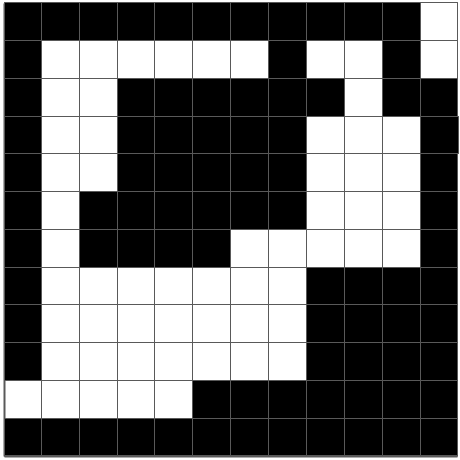
\includegraphics[width=.9\linewidth]{pic/vorwissen/2c_occupgridmap.png}
    \caption{Einfärben der besetzten Kästchen}
  \end{subfigure}
  \caption{Erstellen einer Occupancy Grid Map}
  \label{fig:occupanygridmap}
\end{figure}
\mbox{}


\section{Sensorik}\label{sec:Sensorik}
\addtocontents{toc}{\vspace{0.8cm}}
Die Sensorik eines mobilen Roboters kann unterteilt werden in interne- und externe Sensoren. Die internen Sensoren befinden sich innerhalb des Systems, und umfassen meistens Beschleunigungs-, Gyro- und gegebenenfalls Magnetometer Sensoren, welche für gewöhnlich in einer sogenannten \textit{Internal Measurement Unit} (IMU) zusammengefasst werden. Sie können genutzt werden, um ohne Wissen über die Außenwelt Aufschluss über die Position des Roboters über die Zeit zu geben.\\
Zur Wahrnehmen der Umwelt kommen die externen Sensoren zum Einsatz. Sie erfassen den Raum in dem der Roboter sich aufhält durch beispielsweise Kameras, Ultraschallsensoren oder Laser-Range-Scanner.


\section{\textit{Motion-Model}}\label{sec:Motion-Model}
\addtocontents{toc}{\vspace{0.8cm}}
\begin{wrapfigure}{R}{0.5\textwidth}
    \centering
    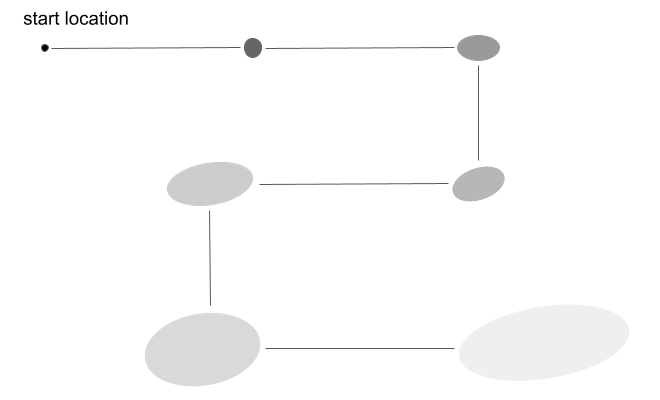
\includegraphics[width=0.45\textwidth]{pic/vorwissen/3b_growinguncertainty.png}
    \caption{wachsende Wahrscheinlichkeitsverteilung über die Aussage der Position des Roboters}
    \label{fig:3b_growing_uncertainty}
\end{wrapfigure}
Die internen Sensoren können in einem sogenannten \textit{Motion-Model} \cite{youtube:motion_model} genutzt werden, um Aufschluss über die aktuelle Position, im Hinblick auf die vorherige Position und das dann ausgeführte Kommando, zu geben. Dieses Motion-Model kann zusammengefasst werden durch $p(x_t|u_t, x_{t-1})$, wird aufgrund externen- oder internen Störfaktoren und wegen Ungenauheiten beziehungsweise Toleranzen in den Messungen der internen Sensoren verwendet. Deshalb werden die Messungen der Sensoren immer mit ein wenig Rauschen modelliert. Üblicherweise wird entweder Gaussch'es Rauschen oder individuell System-abhänigiges Rauschen verwendet. Es wird unterschieden zwischen dem Odometry-basierenden- und dem Geschwindigkeits-basierenden Motion-Model. Im Geschwindigkeits-basierenden Ansatz werden die Daten der IMU verwendet, um eine neue Position durch die vorherige Position und die daraufhin aufgenommenen Geschwindigkeiten zu errechnen. Dieses Vorgehen nennt man auch \textit{dead reckoning}.\\
Der Odometry-basierende Ansatz nutzt zusätzlich zu der IMU Encoder an den Motoren, die das Kommando zur Bewegung ausführen. Der neue Standort wird aus der vorherigen Position, den von den Motoren ausgeführten Umdrehungen und der Physik des Roboters berechnet. Die IMU kann in einer Art Feedback-Schleifen eingebaut werden, um Störungsfaktoren in der Durchführung der Bewegung wahrzunehmen. Die Daten aus der IMU und den Motor-Encodern können dann in einem sogenannten \textit{Kalman Filter} oder \textit{Extendet Kalman Filter} vereint werden. Dieser verrechnet die beiden Messungen mit einer dynamischen Gewichtung, um eine Odometry zu erhalten.\\
Im Beispiel kann man sich das Ergebnis des Motion-Models in etwas so vorstellen:\\
Man gibt einem mobilen Roboter das Kommando, sich 5 Meter vorzubewegen. Durch externe Störfaktoren, wie in etwa Bodenwellen, und interne Störungsfaktoren, wie beispielsweise eine ungleiche Gewichtsverteilung oder das Rutschen von einem Rad, kann die Bewegung "5 Meter nach vorne fahren" vielleicht nicht genau ausgeführt werden. Das Motion-Model gibt jetzt Aufschluss darüber, wie wahrscheinlich es ist, dass der Roboter beispielsweise nur 4,8 meter vorgefahren ist.\\
Wird nur das Motion-Model genutzt um den Standort eines mobilen Roboters festzustellen, kommt es mit zunehmender Zeit und zunehmendem Weg zu einer immer größer werdenden Wahrscheinlichkeitsverteilung, die eine immer geringere Aussagekraft über den tatsächlichen Standort des Roboters hat. (siehe Bild \ref{fig:3b_growing_uncertainty}



\section{\textit{Observation-Model}}\label{sec:Observation-Model}
\addtocontents{toc}{\vspace{0.8cm}}
% TODO Observation-Model
Das Ziel des \textit{Observation Model} \cite{youtube:observation_model} ist Berechnung der Wahrscheinlichkeit der Messungen an einer bestimmten Position in einer bestimmten Welt. Das kann dargestellt werden durch $p(z_t|x_t, m)$, also die Wahrscheinlichkeit $p$ der Messungen $z$ zum Zeitpunkt $t$, gegeben dem Standort $x_t$ in der Karte $m$. Ein Scan eines Laser-Range Scanners besteht aus K Messungen $z_t =\{z_t^i, ..., z_t^K\}$ von Abständen zu Objekten in der Umgebung. \\
Dann gilt $p_s(z_t|x_t,m)=\prod_{i=1}^K p(z_t^i|x_t,m)$ - die Wahrscheinlichkeit eines Scans $p_s$ an einer bestimmten Position in einer bestimmten Karte, ergibt sich aus dem Produkt der Wahrscheinlichkeiten der einzelnen Messungen.\\
Die Wahrscheinlichkeitsverteilung der einzelnen Messungen, gegeben einer erwarteten Messung können verschieden modelliert werden. Ein Ansatz ist zum Abstand der erwarteten Messung eine Gaussch'e Normalverteilung anzuwenden , und ein wenig Grundrauschen einzufügen, im Falle von unerwarteten Zufällen. Ein ausgefeilterer Ansatz wäre eine Wahrscheinlichkeitsverteilung wie sie in Bild \ref{fig:observation_model} dargestellt ist. Sie ergibt sich aus der Überlagerung mehrerer Modelle. Wie in Bild dargestellt, wird zum Abstand der erwarteten Messung eine Gaussch'e Normalverteilung angewendet und Ein Grundrauschen für unvorhergesehene, zufällige Fälle wird ebenfalls beachtet. Zum Ende der Messweite, also zur maximalen Reichweite der Messung, wird ein großer Balken eingeführt. Im Falle einer größeren Umgebung oder eines Fehlers bei der Messung kann es zu einer Ausgabe des höchstmöglichen Messwerts kommen, was hiermit berücksichtigt wird.\\
Außerdem können sich zwischen der erwarteten Messung und dem Standort des Scanners unerwartete Objekte befinden. Die Wahrscheinlichkeit, dass ein solcher Fall eintritt, nimmt mit abnehmender Distanz zur erwarteten Messung ab. Ein Objekt, dass sich direkt vor dem Scanner befindet, kann durch den Zustand $1\star\star\star$ repräsentiert werden, wobei direkt "vor" der $1$ der Scanner steht und sich direkt "hinter" dem letzten $\star$ der erwartete Messabstand befindet. Der Zustand, dass sich ein Objekt an dritter Stelle befindet, kann dargestellt werden durch $001\star$. Der Zustand hinter dem Objekt, also hinter der $1$, ist irrelevant, weswegen es 8 Fälle gibt in denen der Zustand $1\star\star\star$ erreicht wird, und nur einen Fall gibt, in dem der Zustand $0000$ erreicht wird. Dieses exponentiell abnehmende Verhalten wird im dazu markierten Teil der Wahrscheinlichkeitsverteilung in Bild \ref{fig:observation_model} dargestellt.\\
Mithilfe dieser Wahrscheinlichkeitsverteilung kann an jeder bestimmten Position in einer bestimmten Welt die Wahrscheinlichkeit $p$ der einzelnen Messungen und $p_s$ des Scans, im Hinblick auf die wahren Messungen, errechnet werden.
\begin{figure}[b]
    \centering
    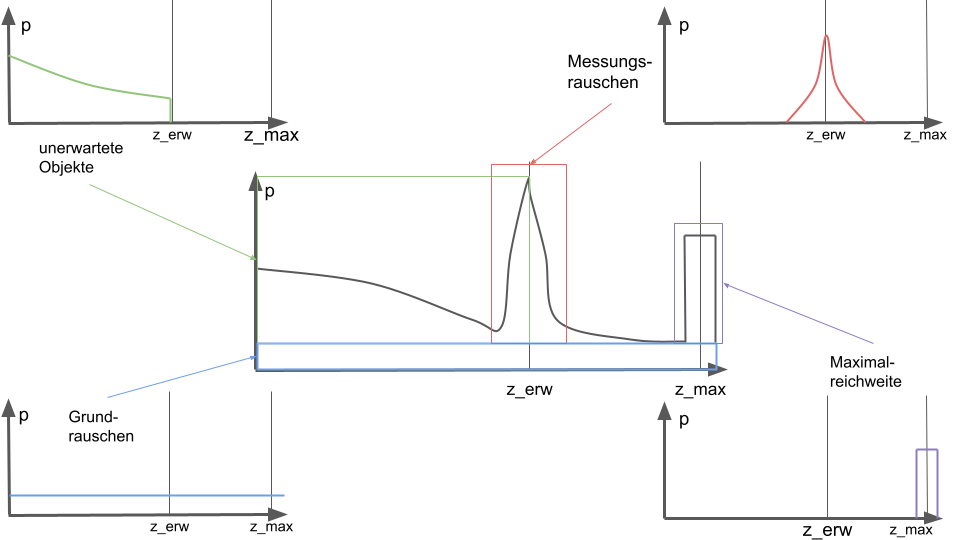
\includegraphics[width=0.9\textwidth]{pic/vorwissen/observation_model.png}
    \caption{ein Observation Model, zusammengesetzt aus Modellen der Gaussch'en Normalverteilung, der Maximalreichweite, den unerwarteten Objekten und den zufälligen Fällen \cite{youtube:observation_model}}
    \label{fig:observation_model}
\end{figure}

